% % % % % % % % % % % % % % % % % % % % % % % % % % % % % % % % % % % % % % % % % % % %
%                                                                                     %
% Short Sectioned Assignment LaTeX Template Version 1.0 (5/5/12)                      %
% This template has been downloaded from: http://www.LaTeXTemplates.com               %
%                                                                                     %
% Original author:  Frits Wenneker (http://www.howtotex.com)                          %
%                                                                                     %
% Modified by: Fco Javier Sueza Rodríguez (fcosueza@disroot.org)                      %
%                                                                                     %
% Changes:                                                                            %
%	    - Custom Chapters, Sections and Subsections (titlesec package)                %
%           - Document type scrbook (oneside)                                         %
%           - Use babel-lang-spanish package and marvosym                             %
%           - Use hyperref, enumitem, tcolorbox and glossaries packages               %
%           - Use Time New Roman (mathptmx), Helvetic and Courier fonts               %
%                                                                                     %
% License: CC BY-NC-SA 3.0 (http://creativecommons.org/licenses/by-nc-sa/3.0/)        %
%                                                                                     %
% % % % % % % % % % % % % % % % % % % % % % % % % % % % % % % % % % % % % % % % % % % %

%-----------------------------------------------%
%	              Packages                  %
%-----------------------------------------------%

\documentclass[paper=a4, fontsize=11pt, oneside]{scrbook}

% ---- Text Input/Output ----- %

\usepackage[T1]{fontenc}
\usepackage[utf8]{inputenc}
\usepackage{mathptmx}
\usepackage[scaled=.92]{helvet}
\usepackage{courier}
\usepackage[indent=12pt]{parskip}

\usepackage{geometry}
\geometry{verbose,tmargin=3cm,bmargin=3cm,lmargin=2.6cm,rmargin=2.6cm}

% ---- Language ----- %

\usepackage[spanish]{babel}
\usepackage{marvosym}

% ---- Another packages ---- %

\usepackage{amsmath,amsfonts,amsthm}
\usepackage{graphics,graphicx}
\usepackage{titlesec}
\usepackage{fancyhdr}
\usepackage{tcolorbox}
\usepackage{hyperref}
\usepackage{enumitem}
\usepackage[automake]{glossaries}

%--------------------------------------------------------------------%
%                      Customizing Document                          %
%--------------------------------------------------------------------%


% ----------- Custom Chapters, Sections and Subsections -------------- %

\titleformat{\chapter}[display]
			{\bfseries\Huge}
			{Tema \ \thechapter} {0.5ex}
			{\vspace{1ex}\centering}

\titleformat{\section}[hang]
			{\bfseries\Large}
			{\thesection}{0.5em}{}

\titleformat{\subsection}[hang]
			{\bfseries\large}
			{\thesubsection}{0.5em}{}

\titleformat{\subsubsection}[hang]
			{\bfseries\large}
			{\thesubsubsection}{0.5em}{}

\hypersetup{
    colorlinks=true,
    linkcolor=black,
    urlcolor=magenta
}

% ------------------- Custom heaaders and footers ------------------- %

\pagestyle{fancyplain}

\fancyhead[]{}
\fancyfoot[L]{}
\fancyfoot[C]{}
\fancyfoot[R]{\thepage}

\renewcommand{\headrulewidth}{0pt} % Remove header underlines
\renewcommand{\footrulewidth}{0pt} % Remove footer underlines

\setlength{\headheight}{13.6pt} % Customize the height of the header

% --------- Numbering equations, figures and tables ----------------- %

\numberwithin{equation}{section} % Number equations within sections
\numberwithin{figure}{section} % Number figures within sections
\numberwithin{table}{section} % Number tables within sections

% ------------------------ New Commands ----------------------------- %

\newcommand{\horrule}[1]{\rule{\linewidth}{#1}} % Create horizontal rule command


%----------------------------------------------------------------------------------------
%	TÍTULO Y DATOS DEL ALUMNO
%----------------------------------------------------------------------------------------

\title{
\normalfont \normalsize
\huge \textbf{Instalación y Configuración de Odoo}
}
\author{Francisco Javier Sueza Rodríguez}
\date{\normalsize\today}

%----------------------------------------------------------------------------------------
%                                     DOCUMENTO
%----------------------------------------------------------------------------------------
\begin{document}

\maketitle

\vspace{2ex}

\begin{center}
    \begin{tabular}{l l}
        \textbf{Centro}: & IES Aguadulce \\
        \textbf{Ciclo Formativo}: & Desarrollo Aplicaciones Web (Distancia)\\
        \textbf{Asignatura}: & Lenguajes de Marcas y Sistemas de Gestión de la Información\\
        \textbf{Tema}: & Tema 1 - Aspectos Básicos de los LM y SGI \\
    \end{tabular}
\end{center}

\vspace{10ex}

\section{Descripción}
En este ejercicio se va a realizar la instalación de un sistema ERP, en concreto de \textbf{Odoo}. Posteriormente, se van a instalar varios módulos, configurando y añadiendo diferente información a cada uno de ellos. La lista de tareas completa es la siguientes:

\begin{enumerate}
    \item \textbf{Instalación y configuración de Odoo}: instalar Odoo ya sea mediante una máquina virtual o usando la versión web.
    \item \textbf{Usuarios}: creación de dos usuarios, uno con datos personales y otro con datos del profesor/a.
    \item \textbf{Informe de productos}: instalar el módulo ``inventario'', crea tres paquetes diferentes y genera un informe de productos creados. Explora el informe en una hoja de cálculo.
    \item \textbf{Petición de mantenimiento}: instala el módulo ``Mantenimiento'' y crea dos peticiones de mantenimiento, una que este en estado ``En Proceso'' y otra en estado ``Reparado''.
\end{enumerate}

\section{Instalación y Configuración de  Odoo}
En primer lugar vamos a instalar Odoo. Nosotros hemos elegido realizar una instalación mediante \textbf{máquina virtual} usando \textbf{VirtualBox}, aunque también se podría hacer una instalación local o usar la prueba online que ofrece Odoo en su web. La instalación de la máquina virtual no la vamos a ver en este documento, por lo que se presupondrá que ya esta instalada.

\subsection{Descarga de la imagen de Odoo}
Primero vamos a descargarnos la imagen de Odoo, la cual podemos encontrar en la \href{https://bitnami.com/stack/odoo/virtual-machine}{página web de Bitnami}, donde encontraremos un archivo con extensión ``\textbf{\textit{.ova}}'' que deberemos descargarnos.

\begin{figure}[h]
    \centering
    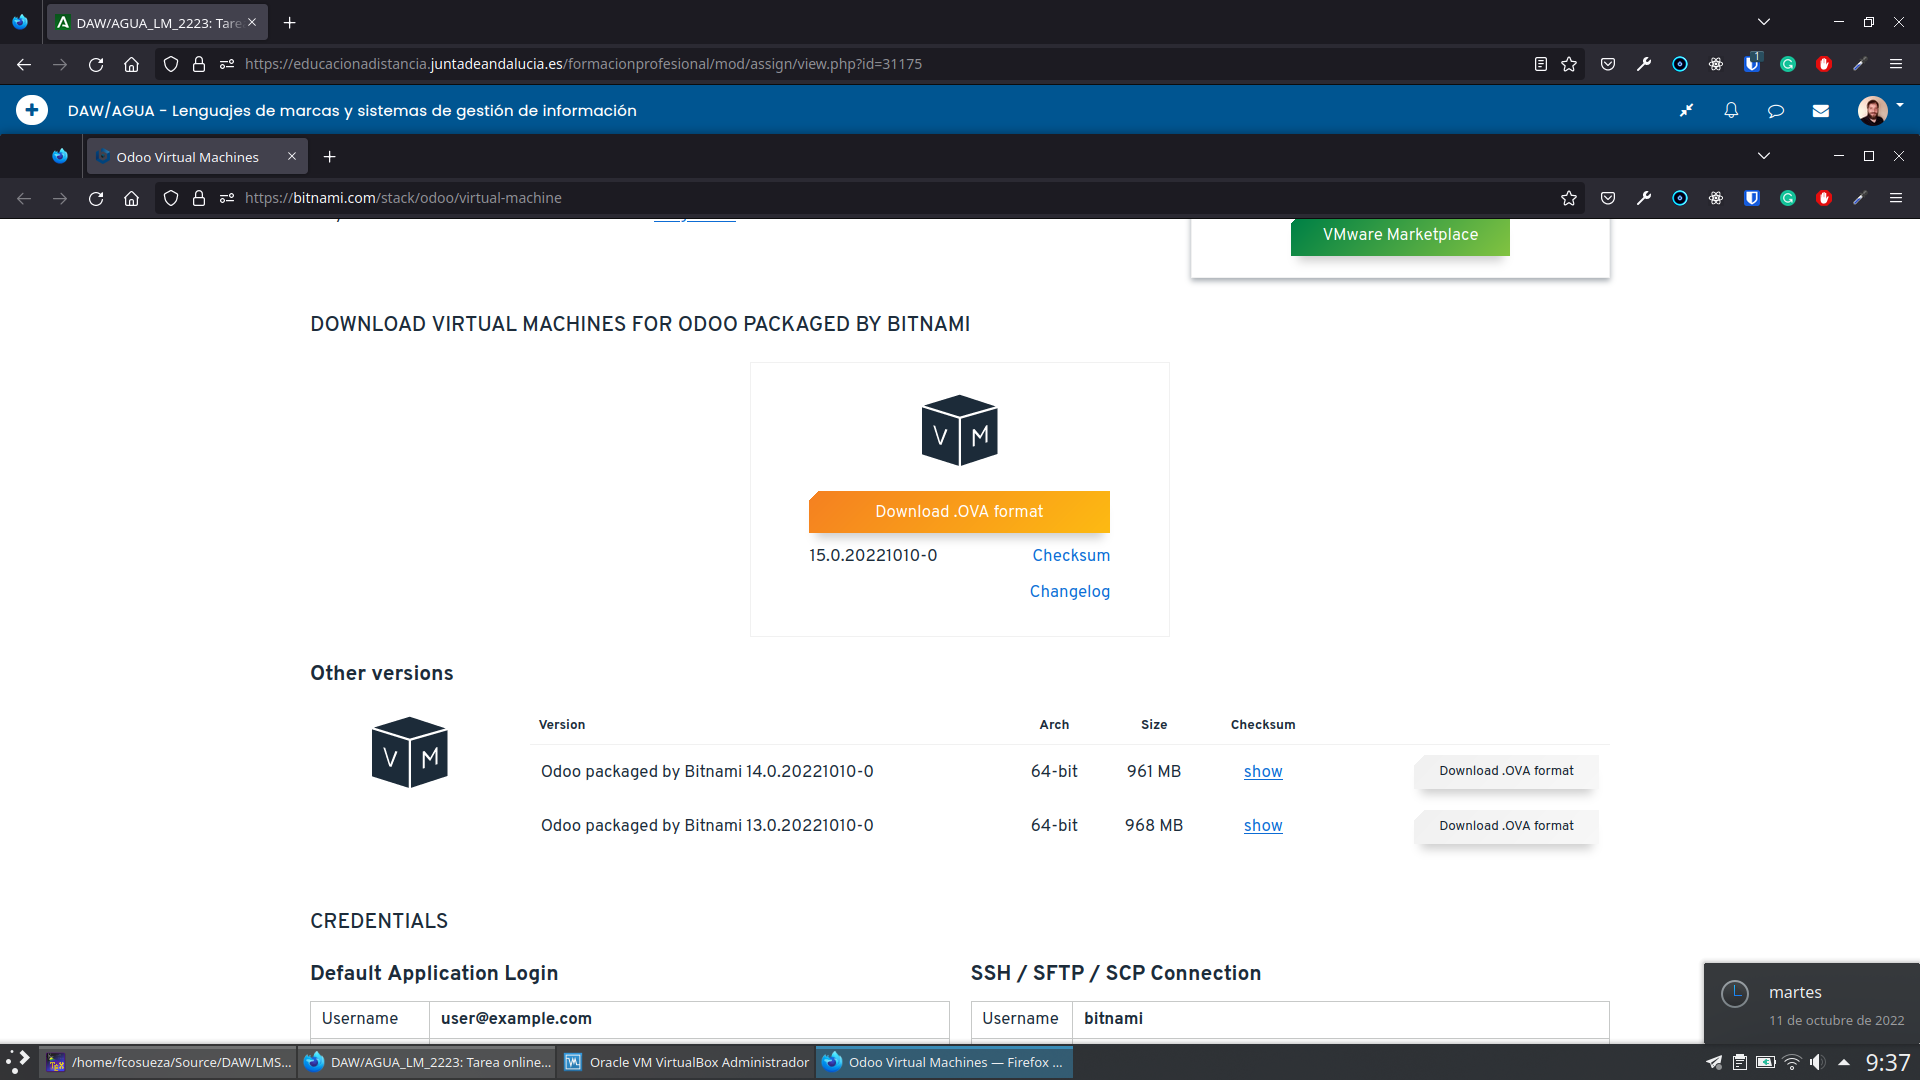
\includegraphics[scale=0.25]{descarga-odoo.png}
    \caption{Página de Bitnami con la imagen de Odoo}
\end{figure}


\subsection{Instalación de la imagen en VirtualBox}
Una vez que tengamos la imagen descargada, tendremos que cargarla en VirtualBox. Para ello, abrimos la aplicaciones y pulsamos el botón importar.

\begin{figure}[h]
    \centering
    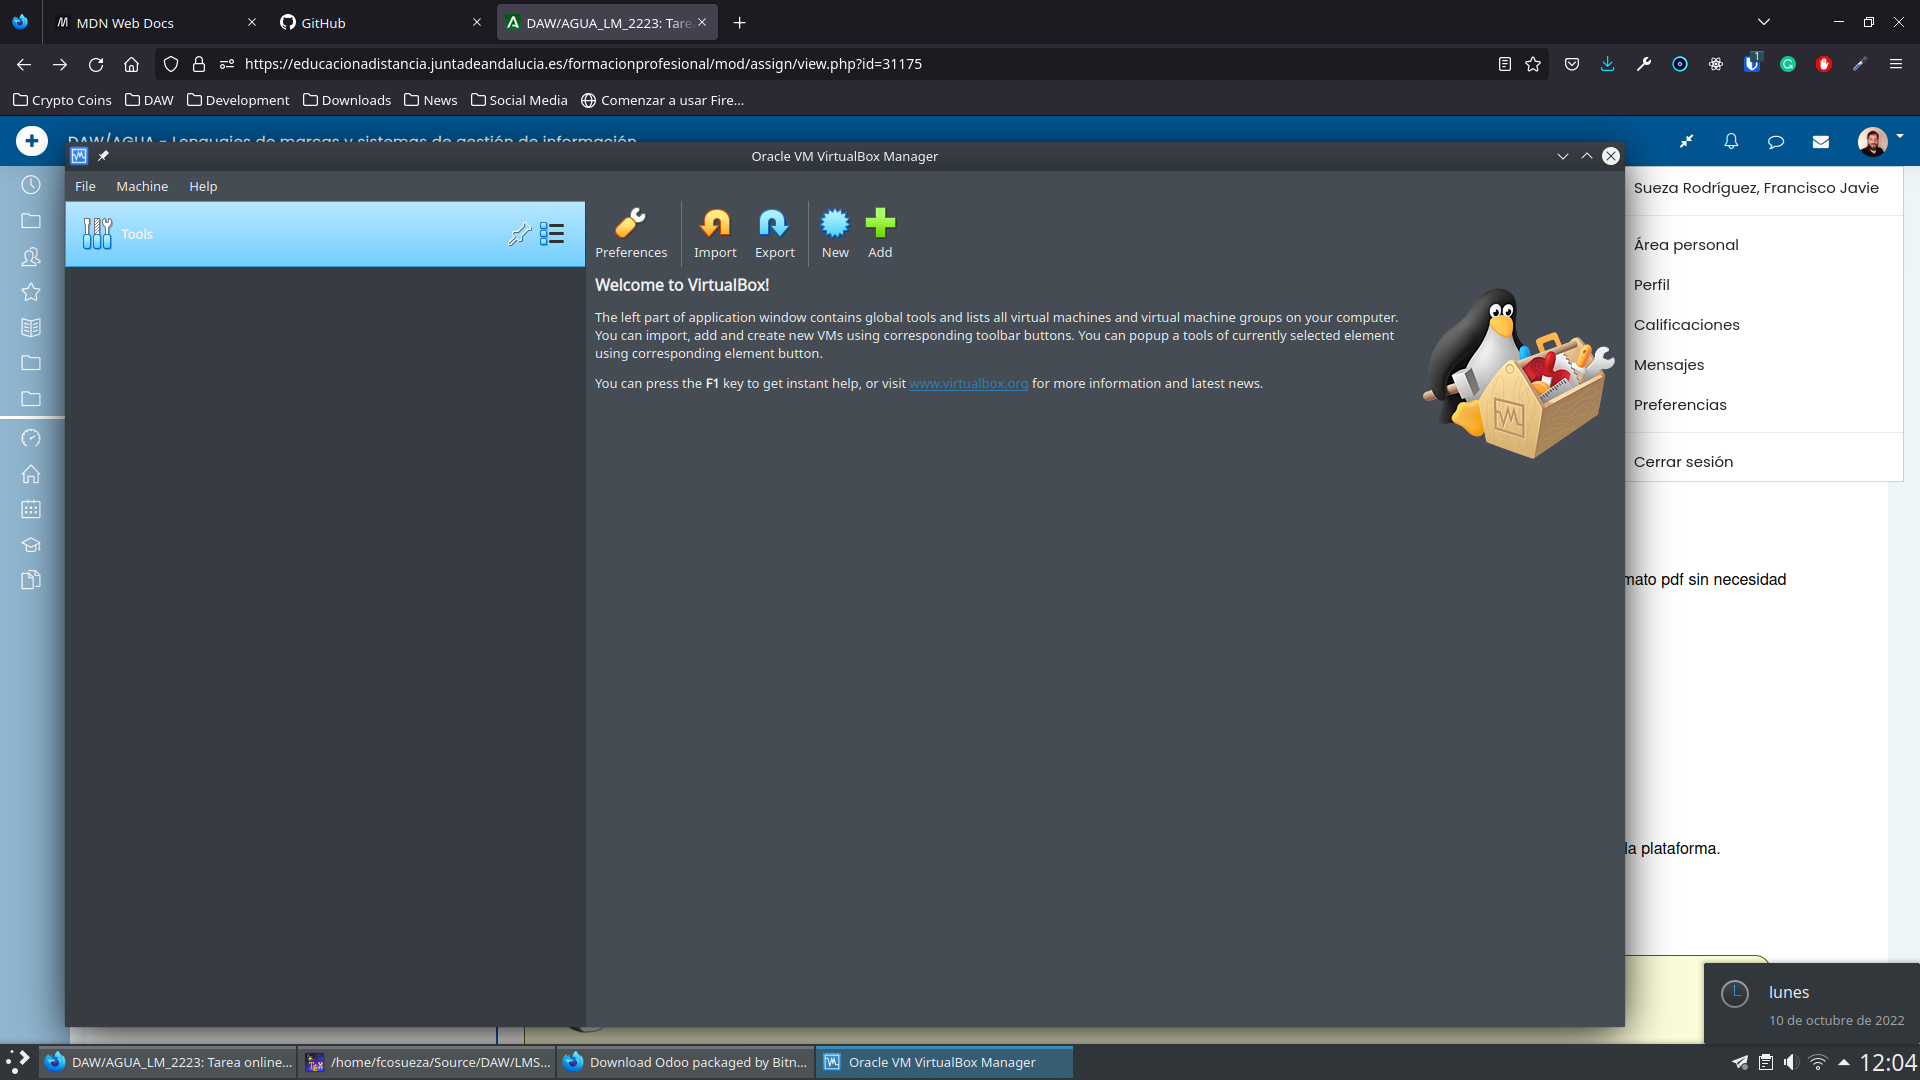
\includegraphics[scale=0.25]{vb-import.png}
    \caption{Pantalla principal de VB}
\end{figure}

A continuación nos saldrá una pantalla donde deberemos seleccionar la imagen que nos hemos descargado y pulsar en siguiente. Una vez seleccionada la imagen, nos mostrará información sobre está, como el tipo de SO, la RAM que utilizará, etc.. Para continuar, deberemos \textbf{pulsar en Importar} de nuevo y la imagen se empezará a cargar en VirtualBox.

Una vez cargada la imagen, ya esta lista para su uso. En la izquierda, tendremos una lista con todas las maquinas virtuales disponibles, en nuestro caso, solo aparece la de Odoo. A la derecha se nos muestra información sobre la máquina virtual seleccionada. Para iniciar la imagen, pulsamos en \textbf{Iniciar}, y comenzará la ejecución de la imagen que hemos descargado.

\begin{figure}[h]
    \centering
    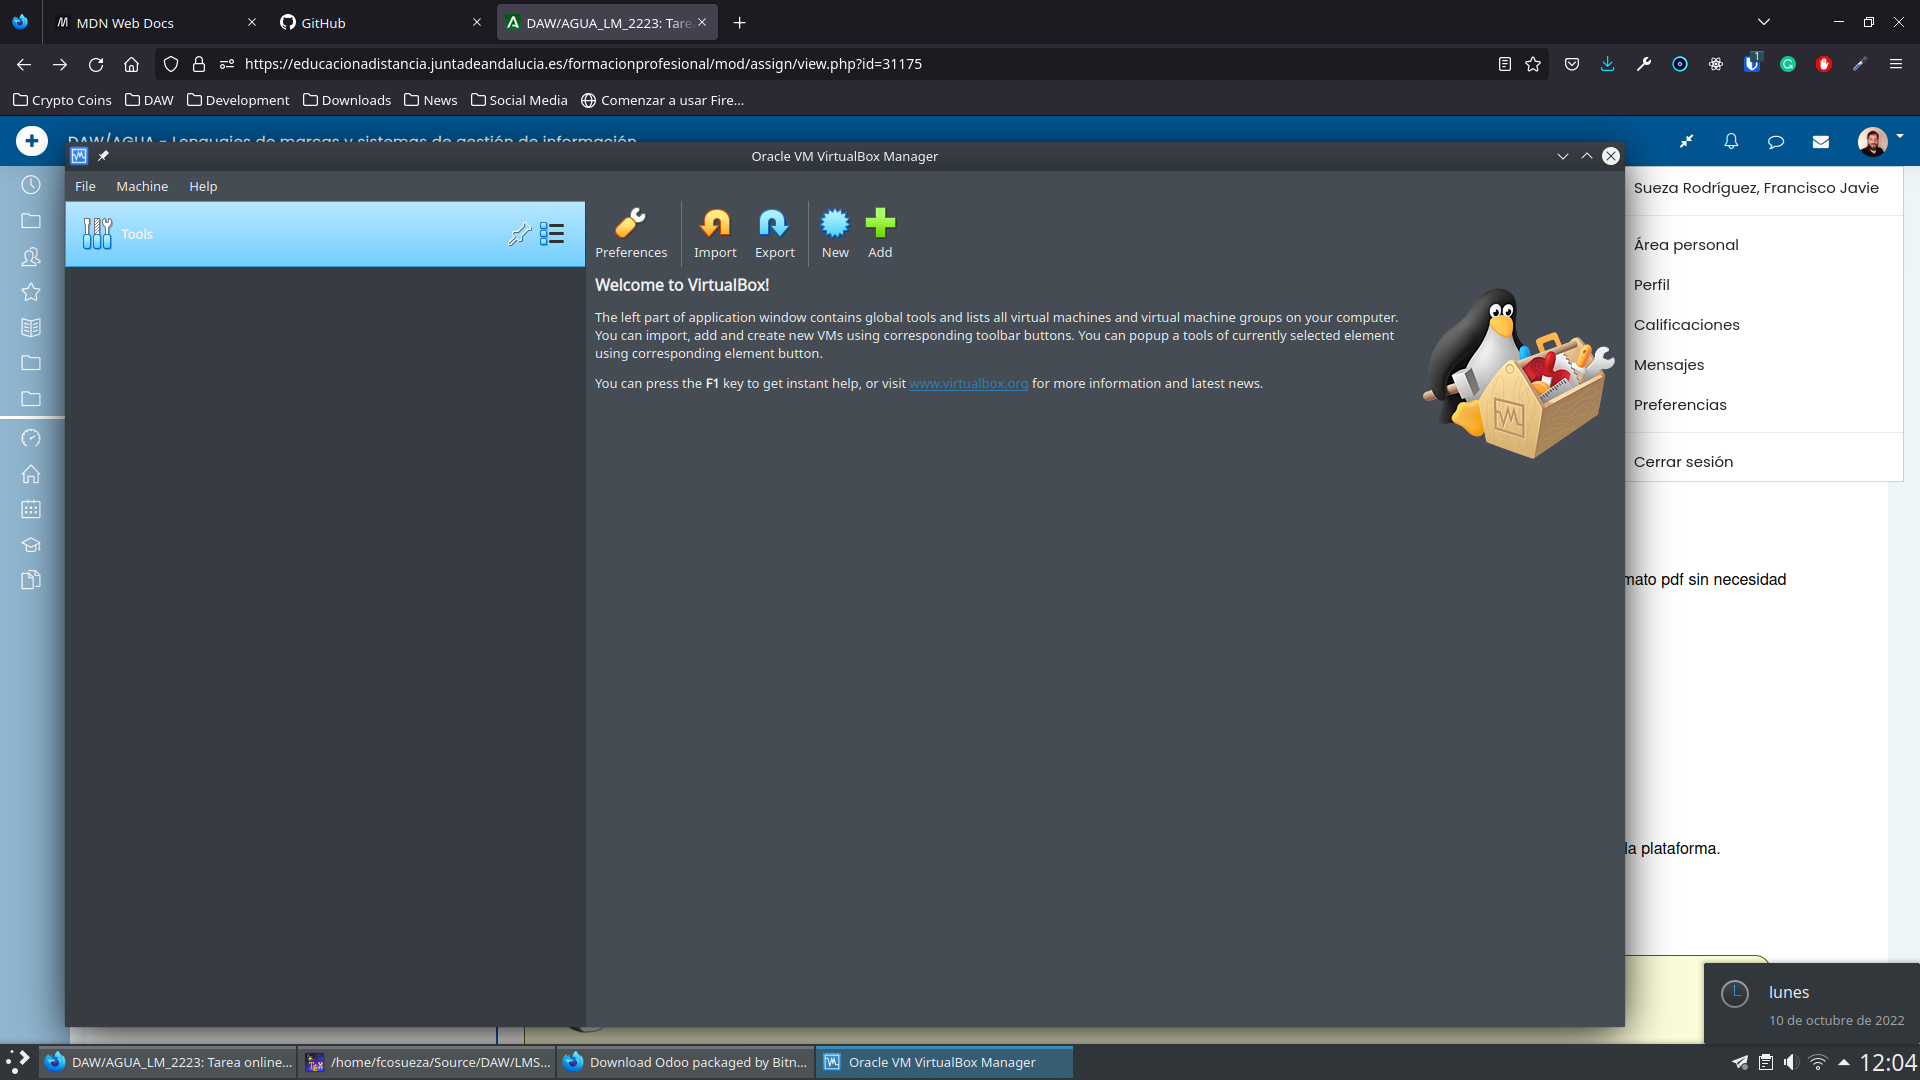
\includegraphics[scale=0.25]{vb-import.png}
    \caption{Información de imagen en Virtual Box}
\end{figure}


\subsection{Accediendo a Odoo}
Cuando hayamos iniciado la imagen de Odoo, nos aparecerá una terminal con información muy importante. Por un lado, nos mostrará la \textbf{dirección del servidor} de Odoo, que nos servirá para acceder a la aplicación desde un navegador. Por otro lado, nos mostrará los credenciales por defecto, \textbf{usuario} y \textbf{contraseña}, que nos servirán para hacer login por primera vez.

\begin{figure}[h]
    \centering
    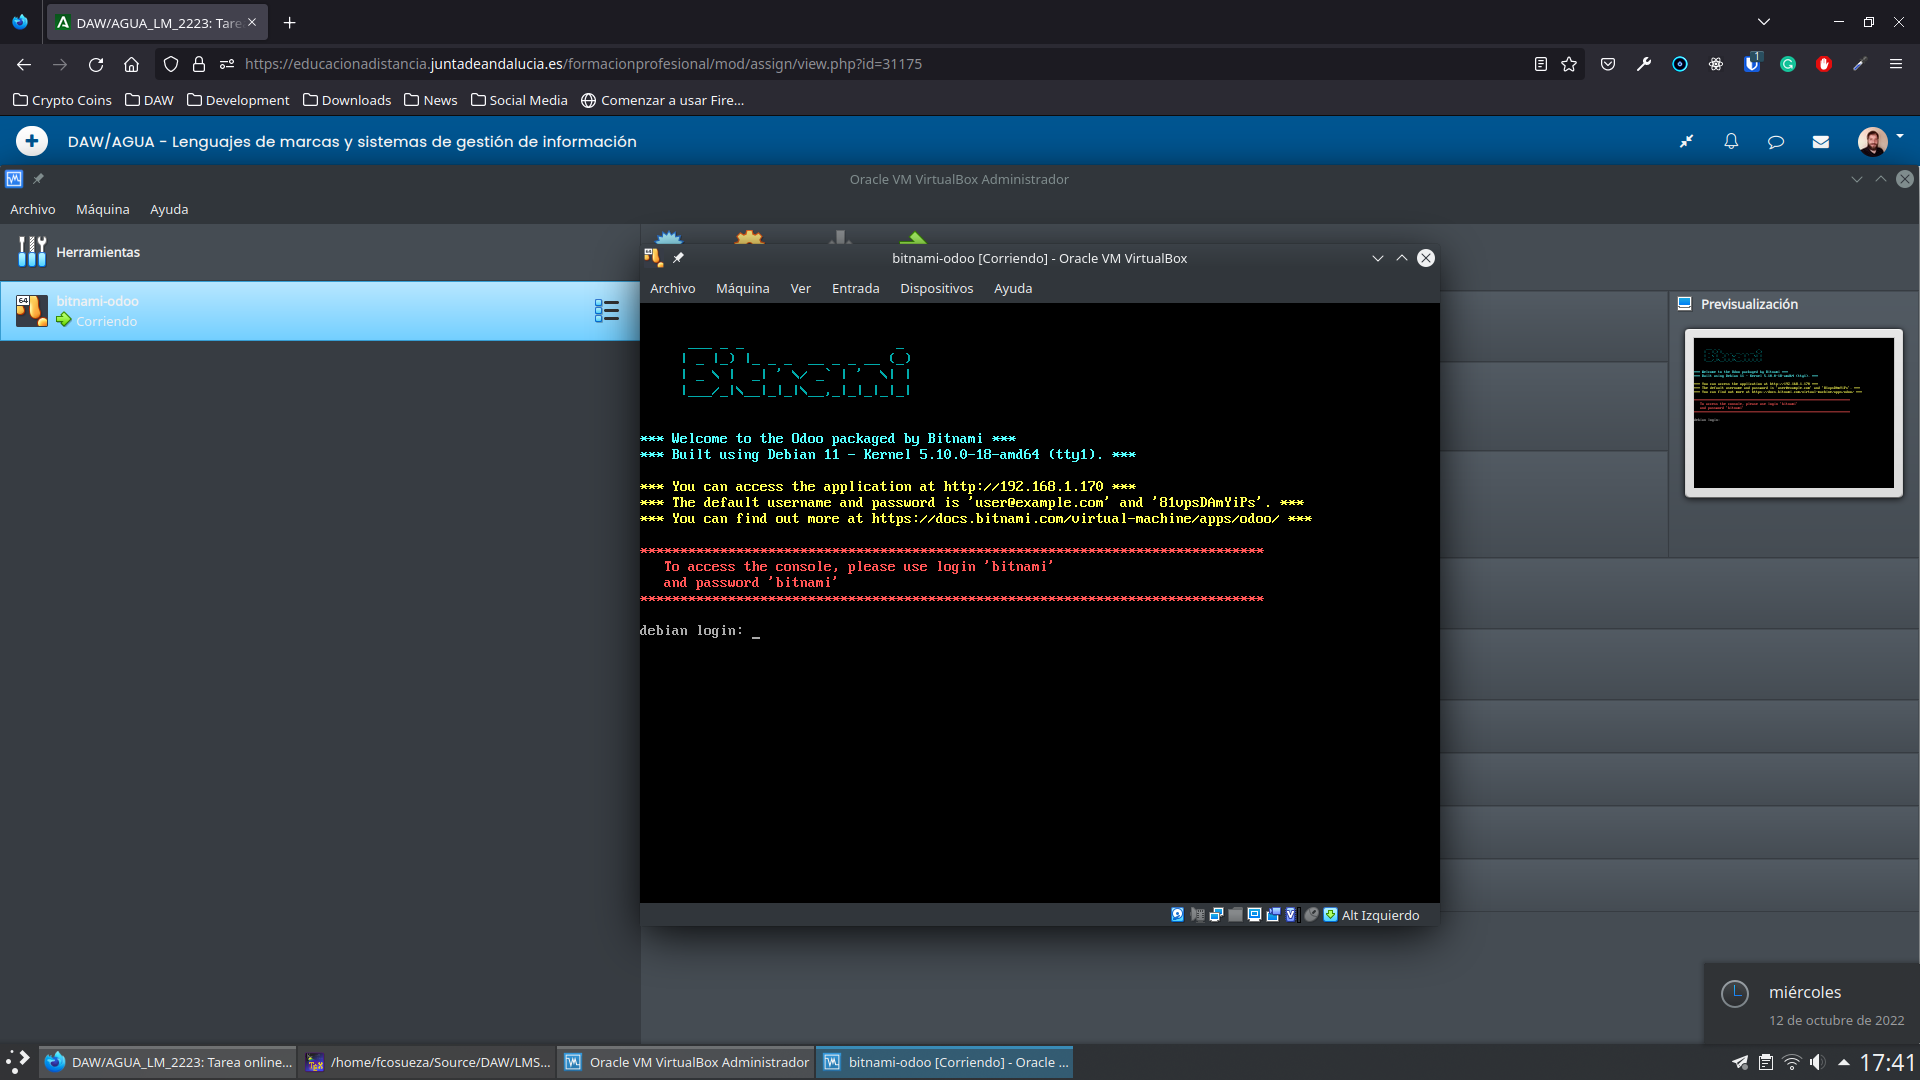
\includegraphics[scale=0.25]{odoo-image-run.png}
    \caption{Terminal inicial de la imagen de Odoo}
\end{figure}

En nuestro caso, la dirección del servidor es \textbf{\textit{http://192.168.1.169}}, mientras que el usuario es \textbf{\textit{user@example.com}} y la contraseña \textbf{\textit{64HBtbt9Iznm}}.

Con estos datos, abrimos un navegador, no importa cual sea, he introducimos la dirección del servidor en la barra de direcciones. Lo que nos mostrará la pantalla inicial de inicio de sesión de Odoo. A continuación introducimos el usuario y la contraseña proporcionados y pulsamos en \textbf{Log in}.


\begin{figure}[h]
    \centering
    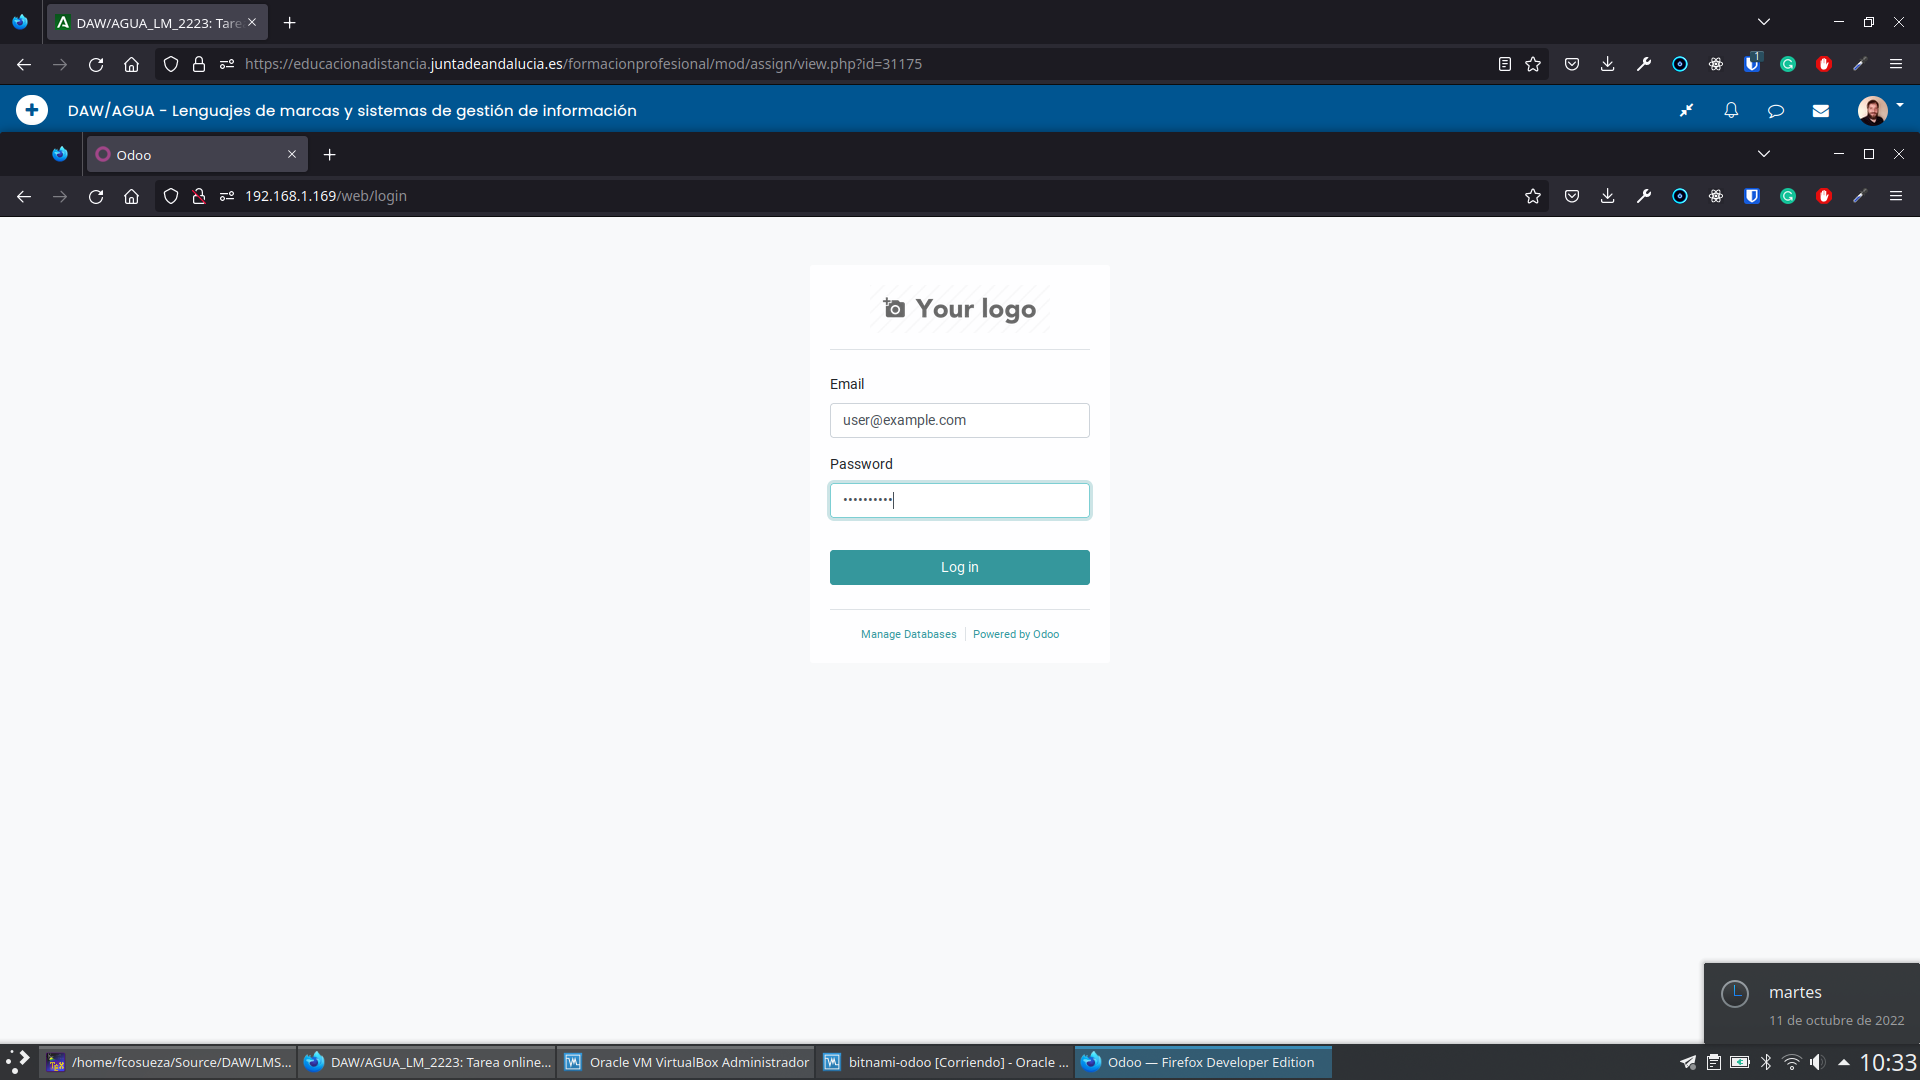
\includegraphics[scale=0.25]{login-odoo.png}
    \caption{Pantalla de inicio de sesión de Odoo}
\end{figure}

\subsection{Cambio de contraseña}
Después de haber iniciado sesión, nos parecerá la pantalla principal de Odoo. Aquí se nos muestran todos los\textbf{ módulos disponibles} para instalar. A la izquierda, podemos \textbf{seleccionar una categoría} y que nos muestre solo los módulos que pertenecen a dicha categoría. Como podemos ver arriba a la derecha, podemos ver que ya se ha creado un \textbf{usuario por defecto}, llamado \textbf{Administrator} y arriba a la izquierda tenemos un \textbf{menú desplegable}.

\begin{figure}[h]
    \centering
    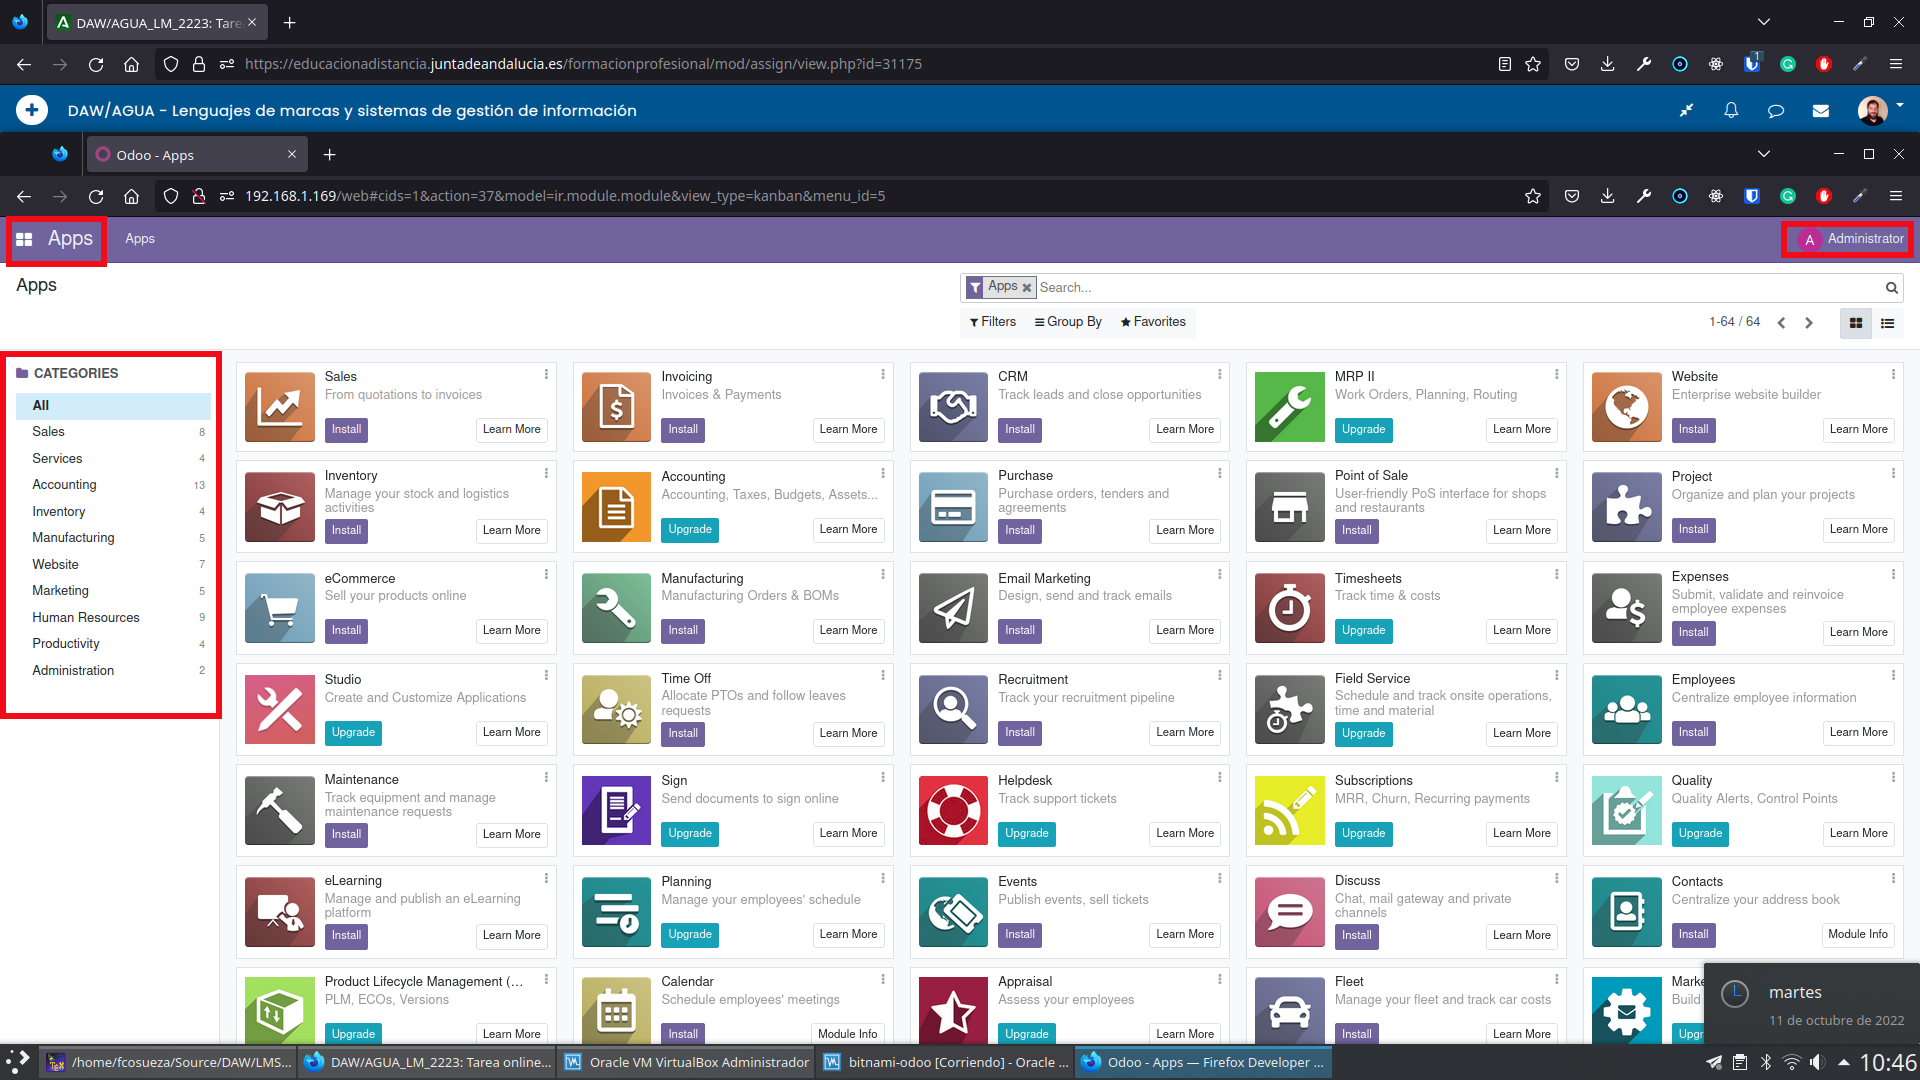
\includegraphics[scale=0.25]{main-odoo.png}
    \caption{Pantalla principal de Odoo}
\end{figure}

Lo primero que deberíamos hacer, es cambiar la contraseña de administrador por la que nosotros queramos. Es conveniente, como en cualquier otra aplicación, utilizar una contraseña fuerte, que sea larga y que alterne números, letra en minúscula y mayúscula, etc..

\begin{enumerate}
    \item Abrimos el menú desplegable, que se encuentra arriba a la derecha, y pulsamos en la opción \textbf{Settings}, que nos abrirá por defecto la pantalla \textbf{Users}.

    \begin{figure}[h]
        \centering
        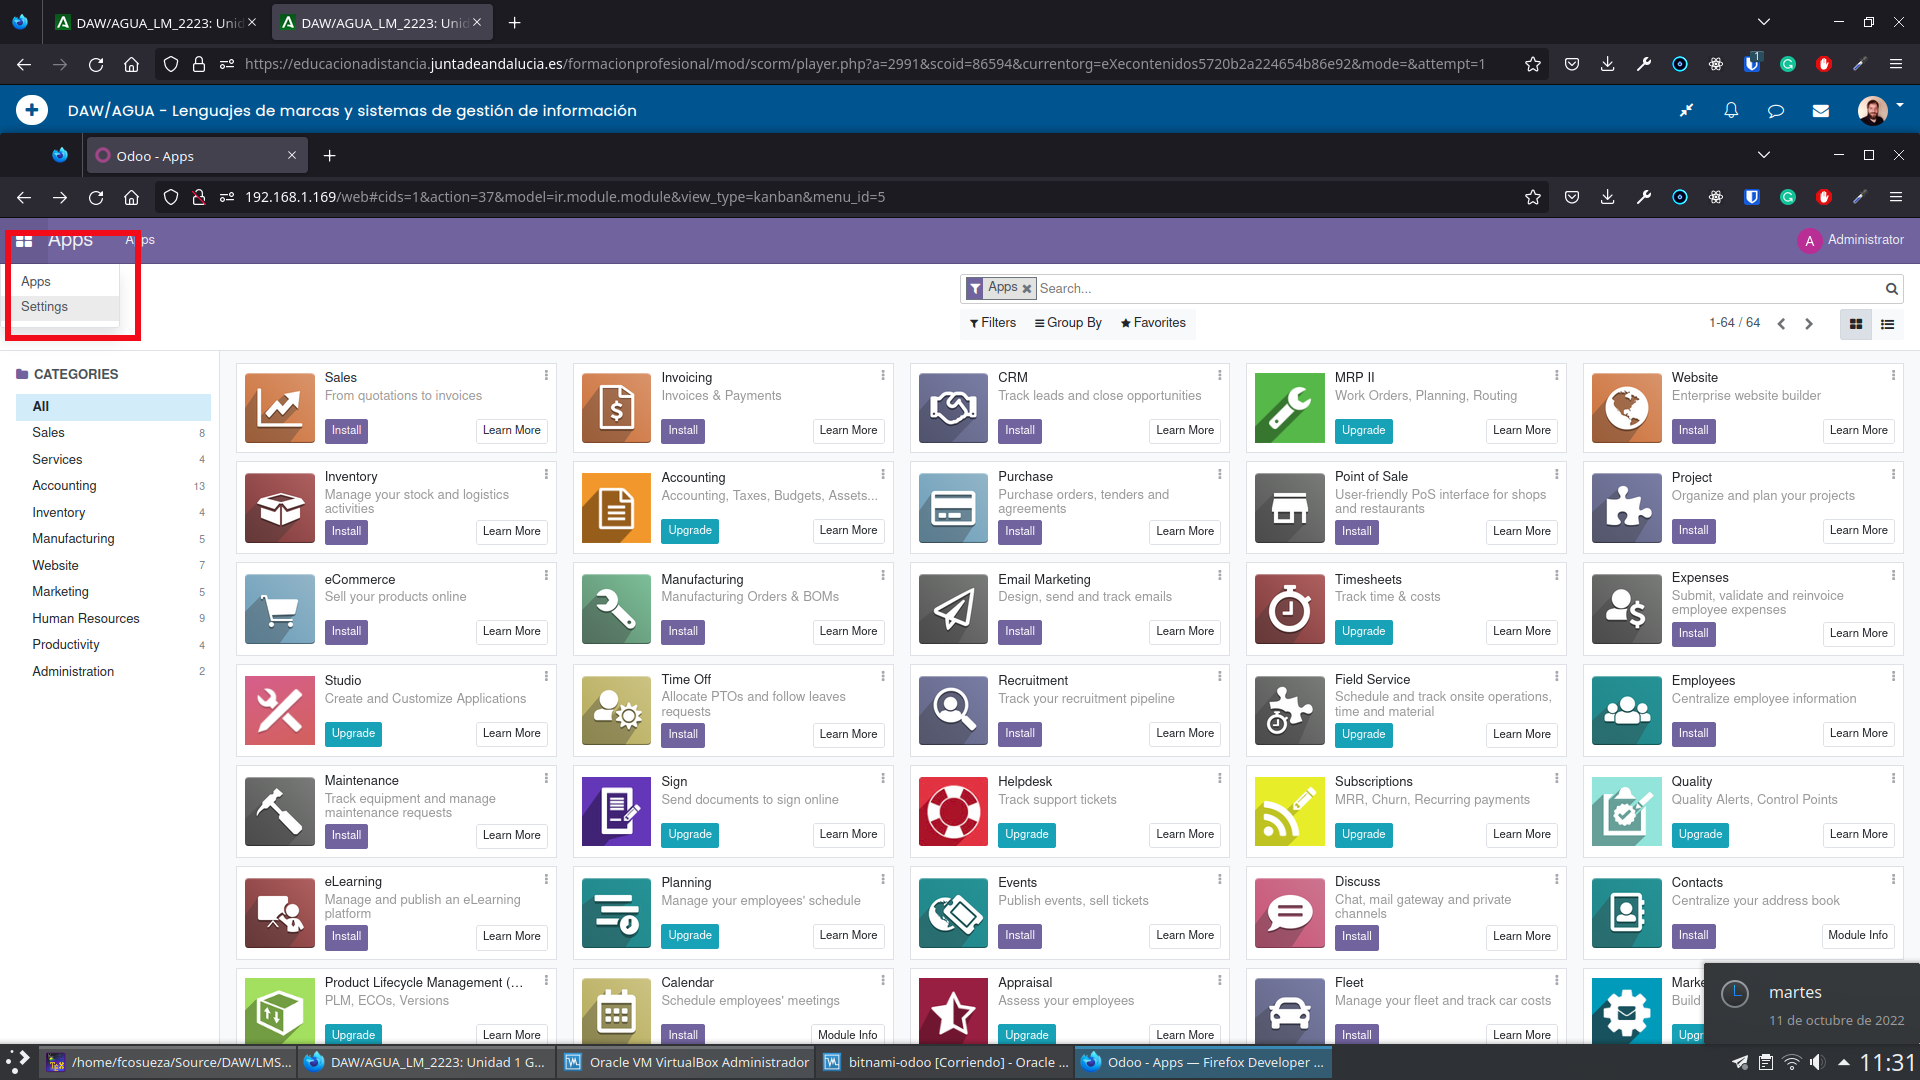
\includegraphics[scale=0.25]{change-pass-01.png}
        \caption{Opción Setting del menú desplegable}
    \end{figure}

    \item En la siguientes pantalla, se nos mostrará la lista de usuarios, en nuestra caso solo tenemos al usuario \textbf{Admnistrator}, seleccionamos este usuario.

    \begin{figure}[h]
        \centering
        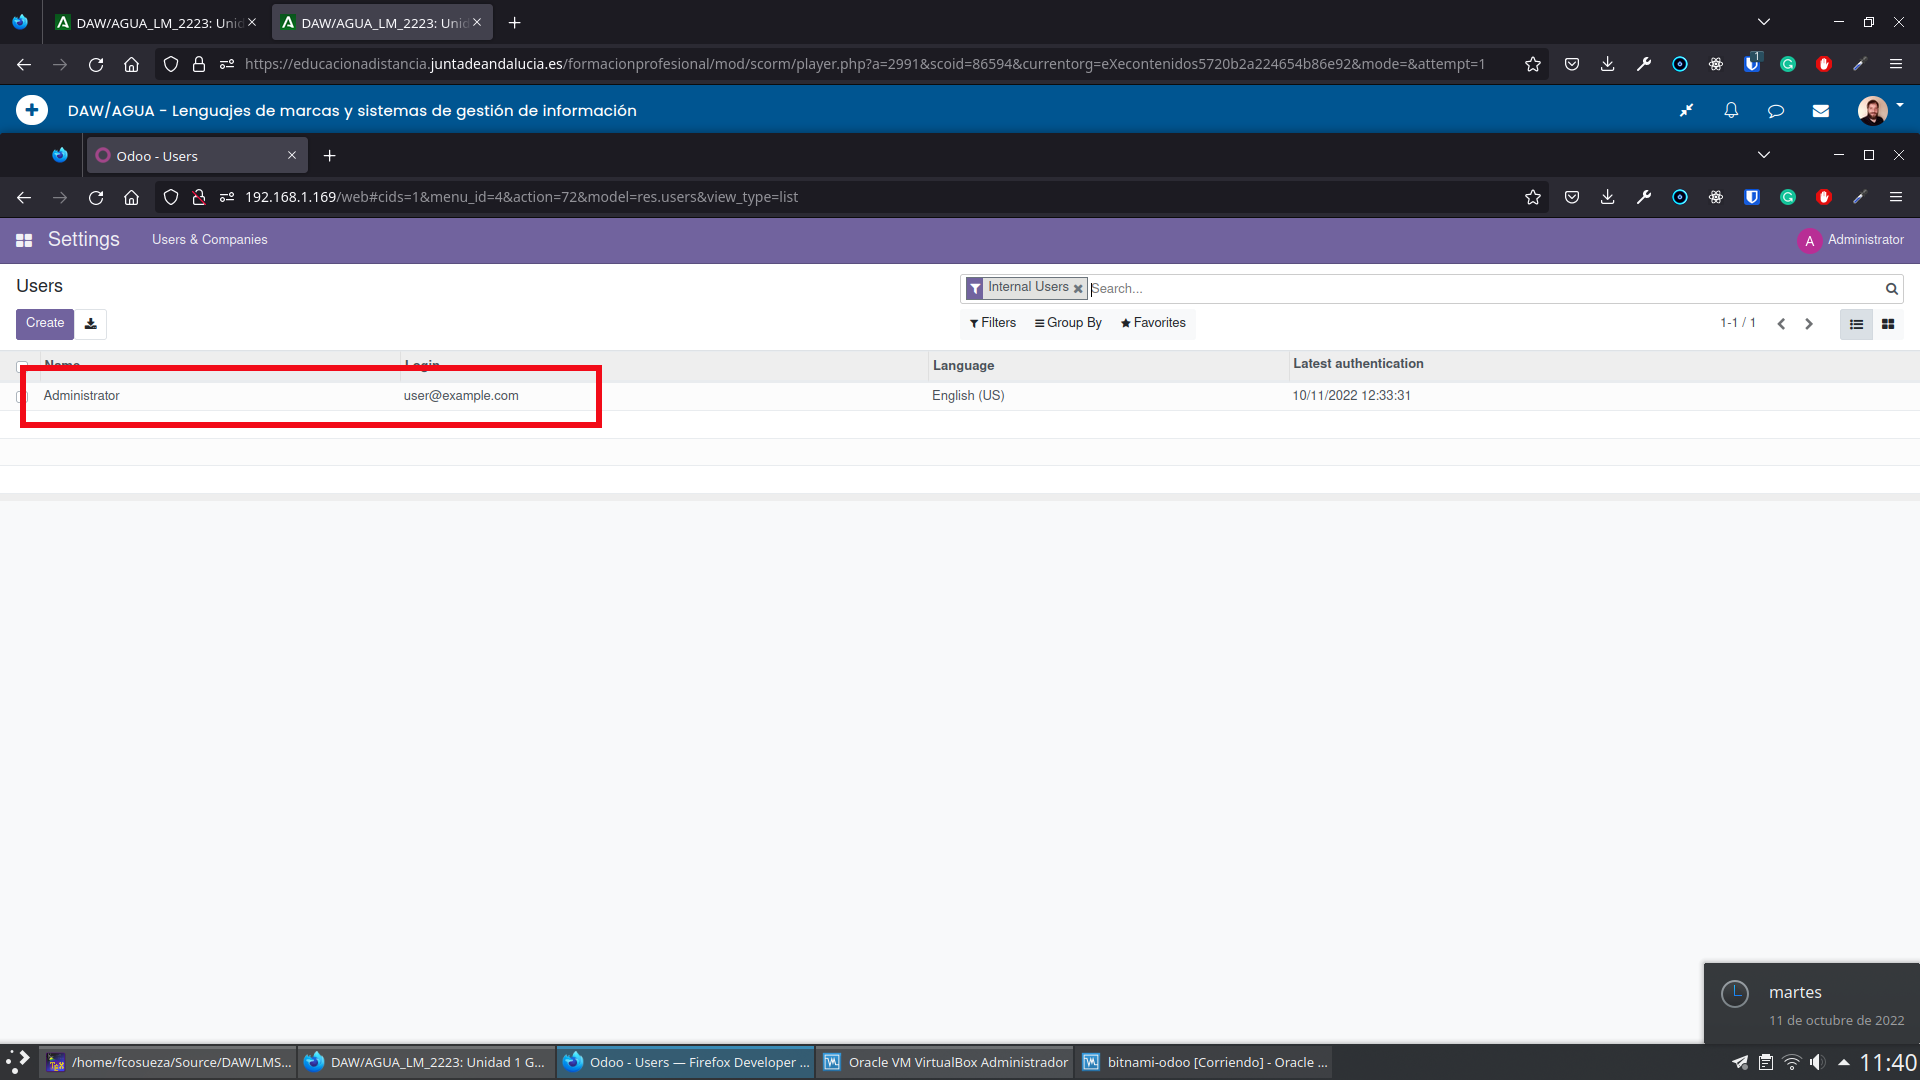
\includegraphics[scale=0.25]{change-pass-02.png}
        \caption{Pantalla de gestión de usuarios de Odoo}
        \label{odoo-users}
    \end{figure}

    \item Una vez hayamos seleccionado el usuario nos mostrará una pagina con un ficha de éste. Se nos mostrará información del usuario, como su correo, el nombre, una foto, en caso de que la tenga, y en la parte inferior los derechos de acceso (Access Rights), las preferencias (preferences) y la configuración de seguridad de la cuenta (Account Security).

    Como a nosotros solo nos interesa, cambiar la contraseña, vamos a desplegar el \textbf{menú Action}, que se encuentra en la parte superior, y seleccionar la opción \textbf{Change Password}.

    \vspace{8ex}

    \begin{figure}[h]
        \centering
        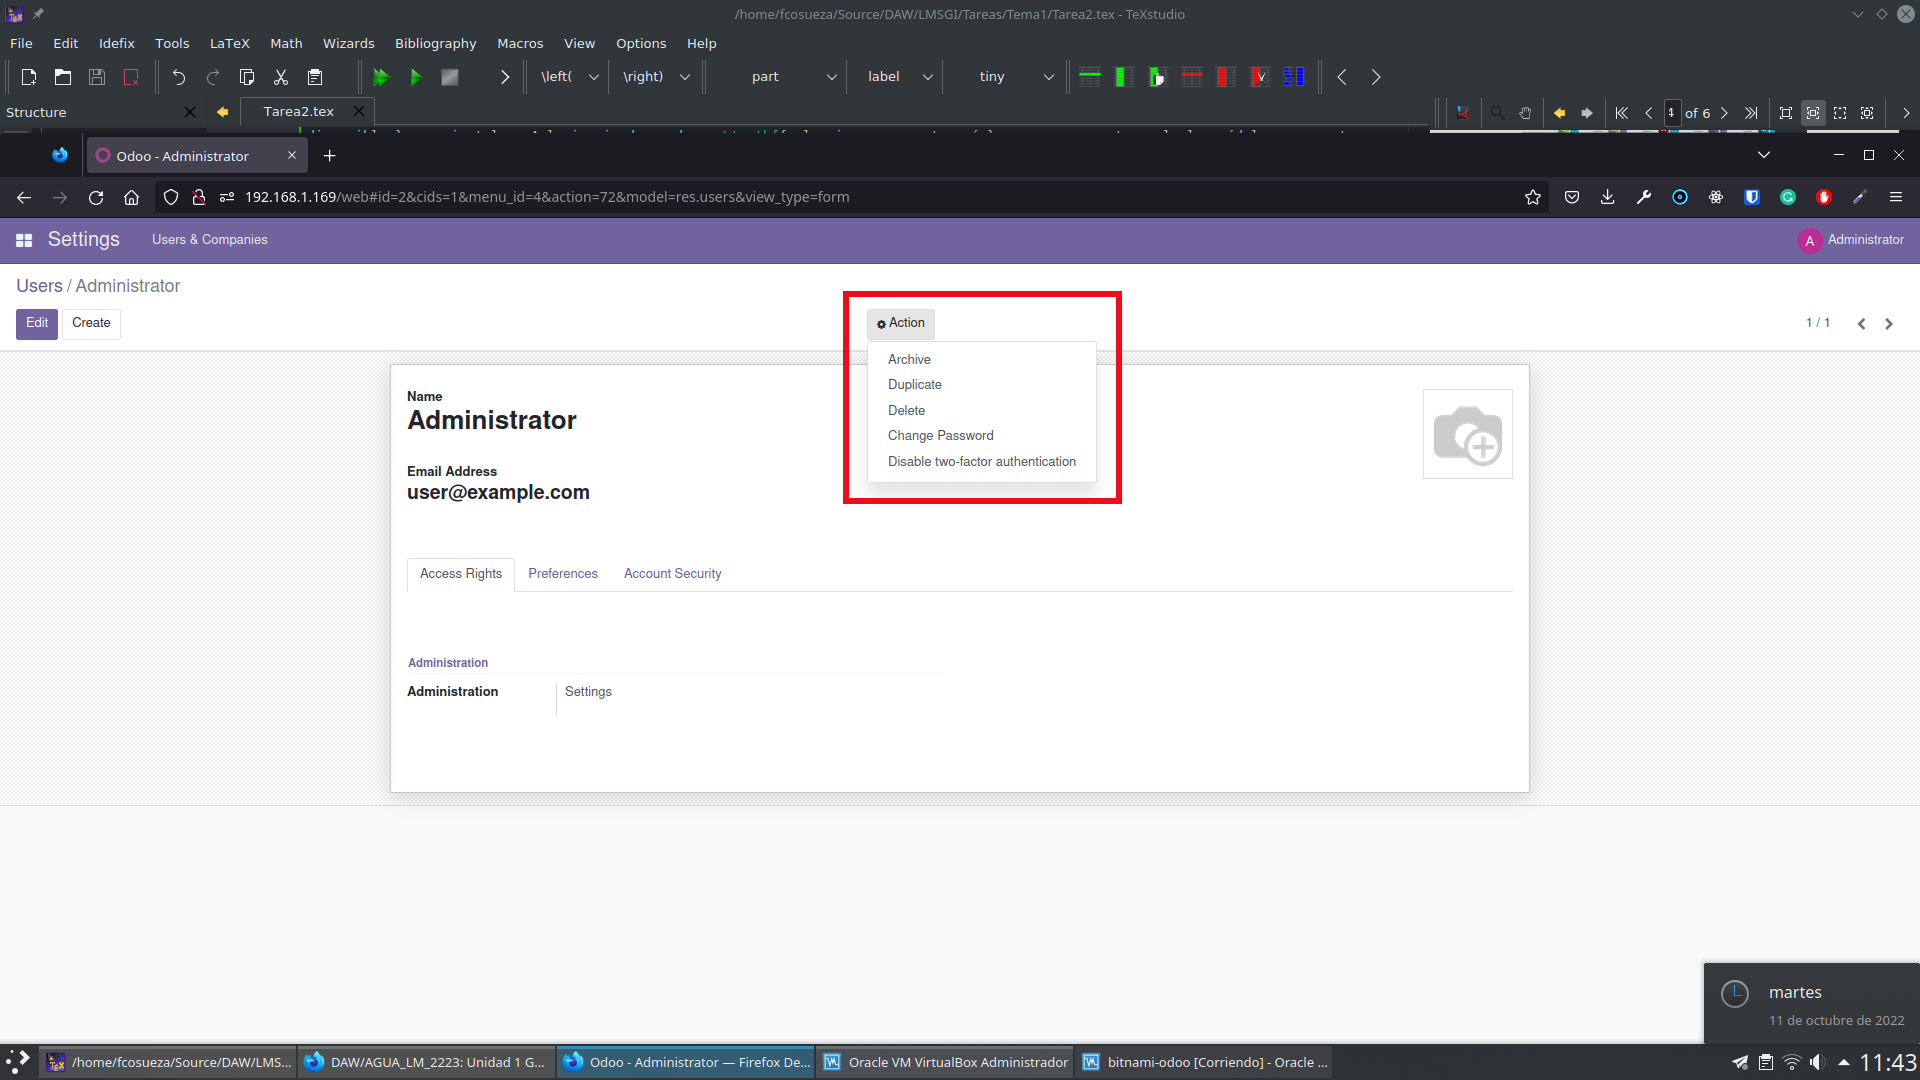
\includegraphics[scale=0.25]{change-pass-03.png}
        \caption{Pantalla con ficha de usuario}
    \end{figure}

    \item A continuación aparecerá una pantalla donde se nos mostrará el usuario y al lado un una entrada de formulario para introducir la nueva contraseña. La introducimos, pulsamos el botón \textbf{Change Password} y se habrá completado el proceso. Tras el cambio, no redirigirá a la pantalla de Log In.

    \begin{figure}[h]
        \centering
        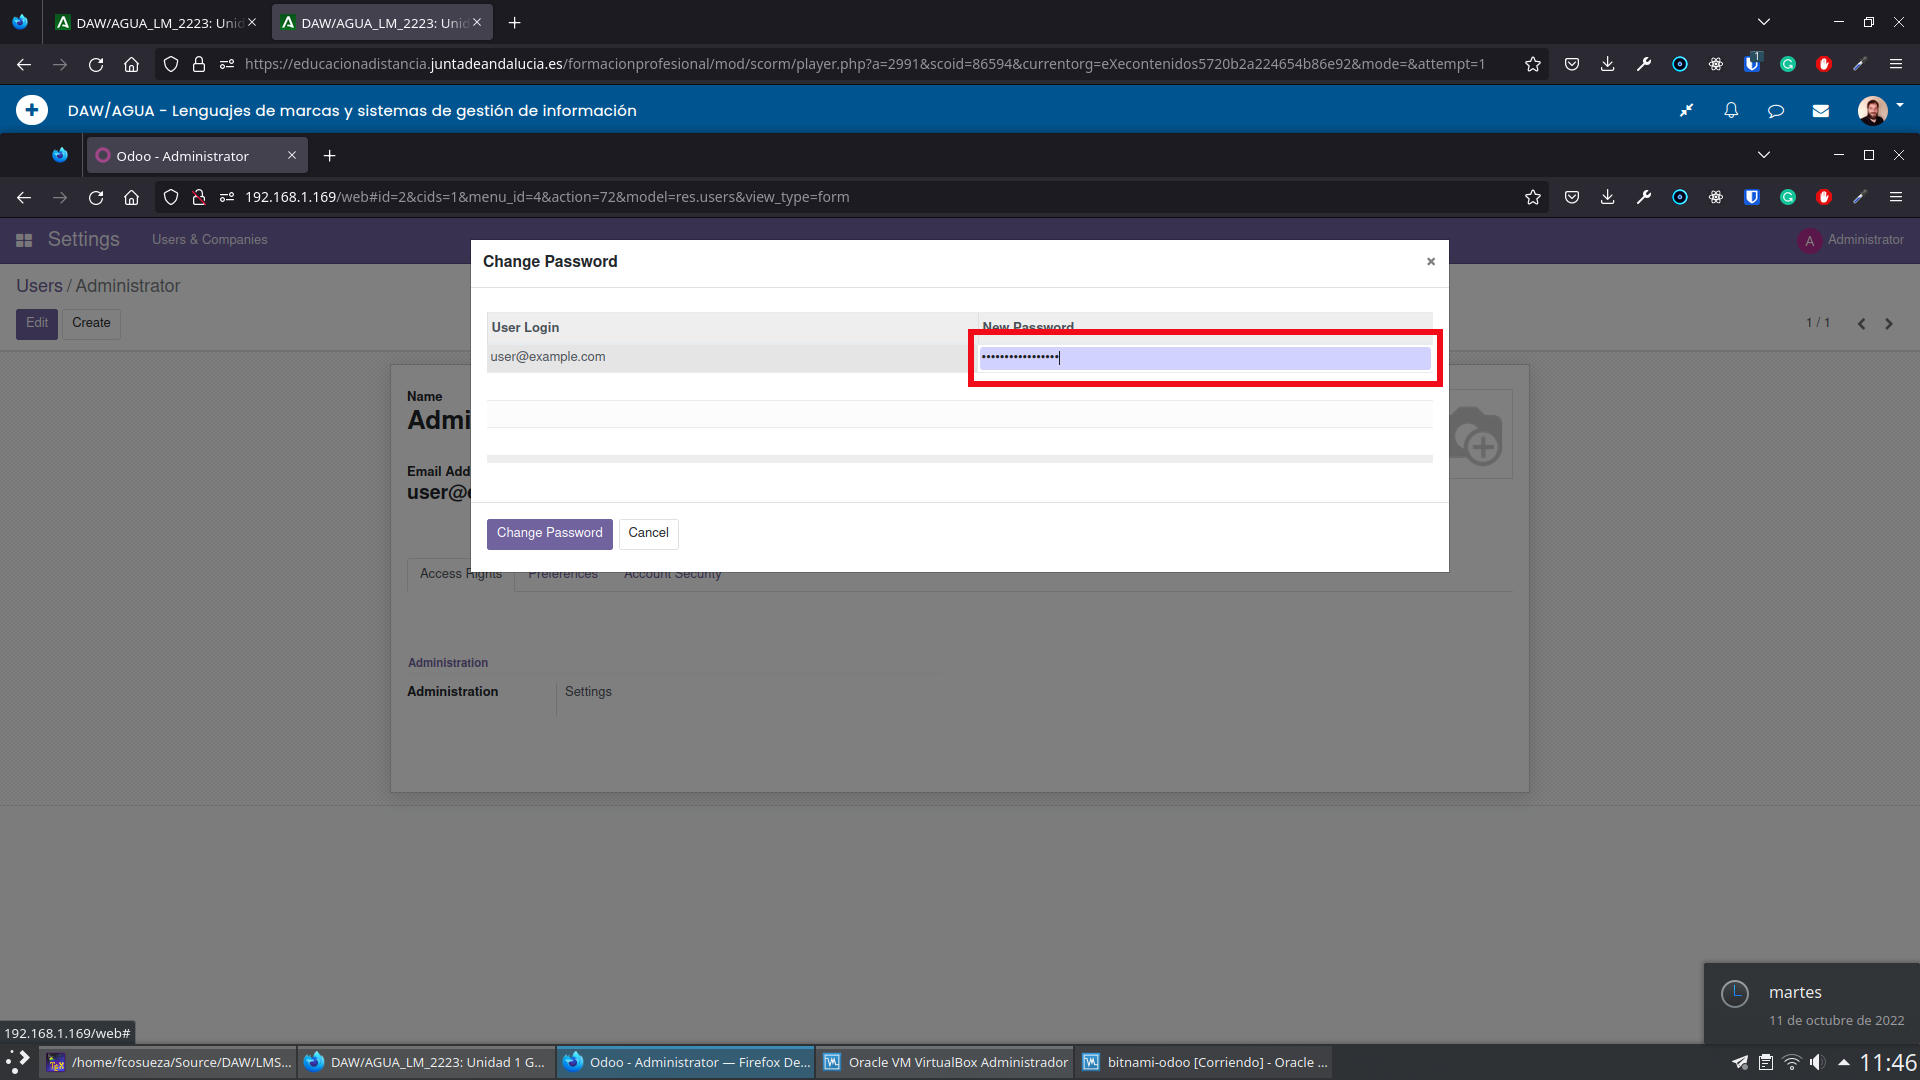
\includegraphics[scale=0.25]{change-pass-04.png}
        \caption{Pantalla de cambio de contraseña}
    \end{figure}
\end{enumerate}

Ya hemos hecho el cambio de contraseña. En la siguiente sección sección veremos como añadir información al sistema y crear nuevos usuarios.

\subsection{Añadiendo Datos de la Empresa}
El último paso para acabar la configuración inicial es añadir los datos de la empresa. En nuestro caso, vamos a rellenarlos con la empresa ficticia \textbf{Llegaya}, añadiendo \textbf{nombre}, \textbf{dirección}, \textbf{teléfono}, \textbf{lema de la empresa}, \textbf{sitio web}, \textbf{NIF} y \textbf{email}.

Los pasos a seguir para añadir estos datos son los siguientes:

\begin{enumerate}
    \item Partiendo desde la pantalla que se muestra en la Figura \textbf{\ref{odoo-users}}, desplegamos el menú \textbf{Users and Companies} y seleccionamos la opción \textbf{Companies}.

    \begin{figure}[h]
        \centering
        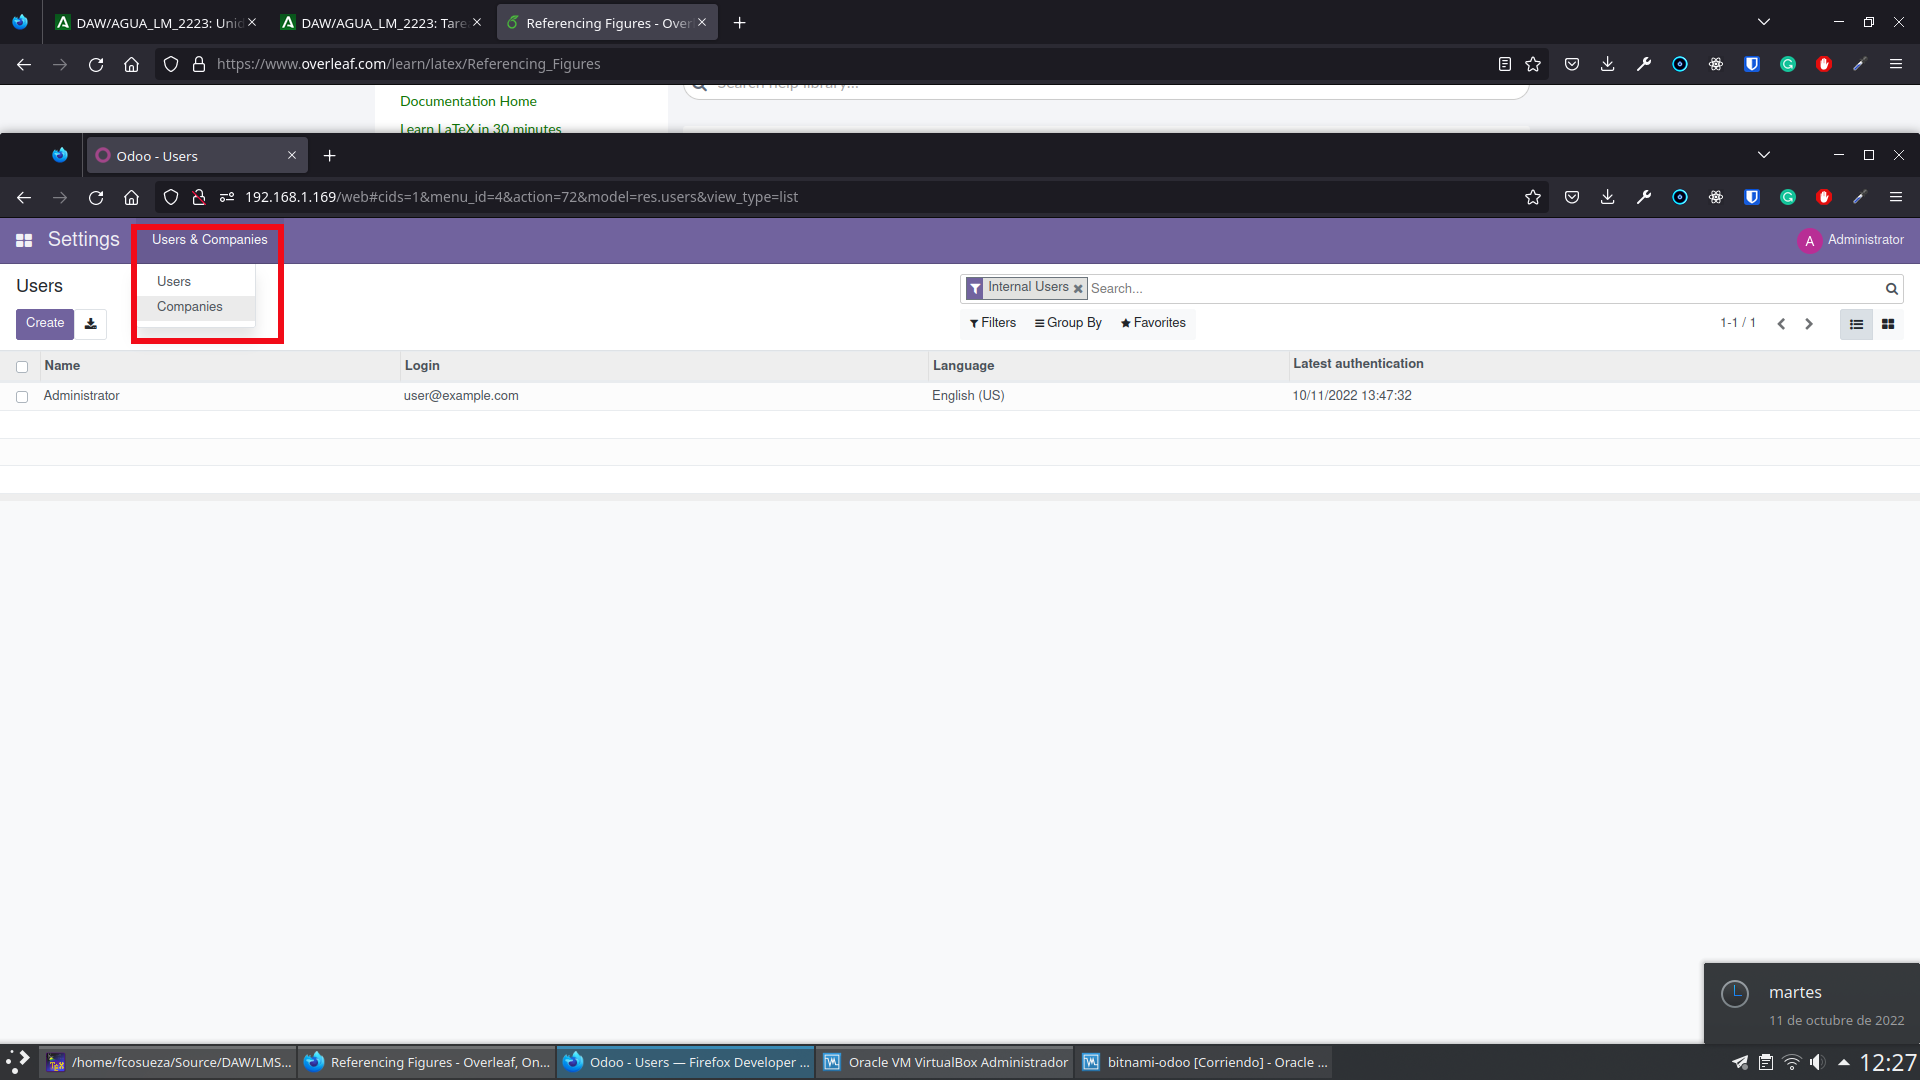
\includegraphics[scale=0.25]{odoo-comp-01.png}
        \caption{Selección menú compañías}
    \end{figure}

    \item A continuación se nos mostrará una pantalla similar a la anterior, pero en vez de con una lista de usuarios, con una lista de compañías. En nuestro caso solo figurará la compañía por defecto \textbf{My Company}. La seleccionamos como hicimos con los usuarios en la sección anterior.

    \item Una vez seleccionada, se nos mostrará una ficha, similar a la de los usuarios, pero con datos de la compañía. Para editarla, pulsamos el botón \textbf{Edit} que se encuentra arriba a la izquierda.

     \begin{figure}[h]
        \centering
        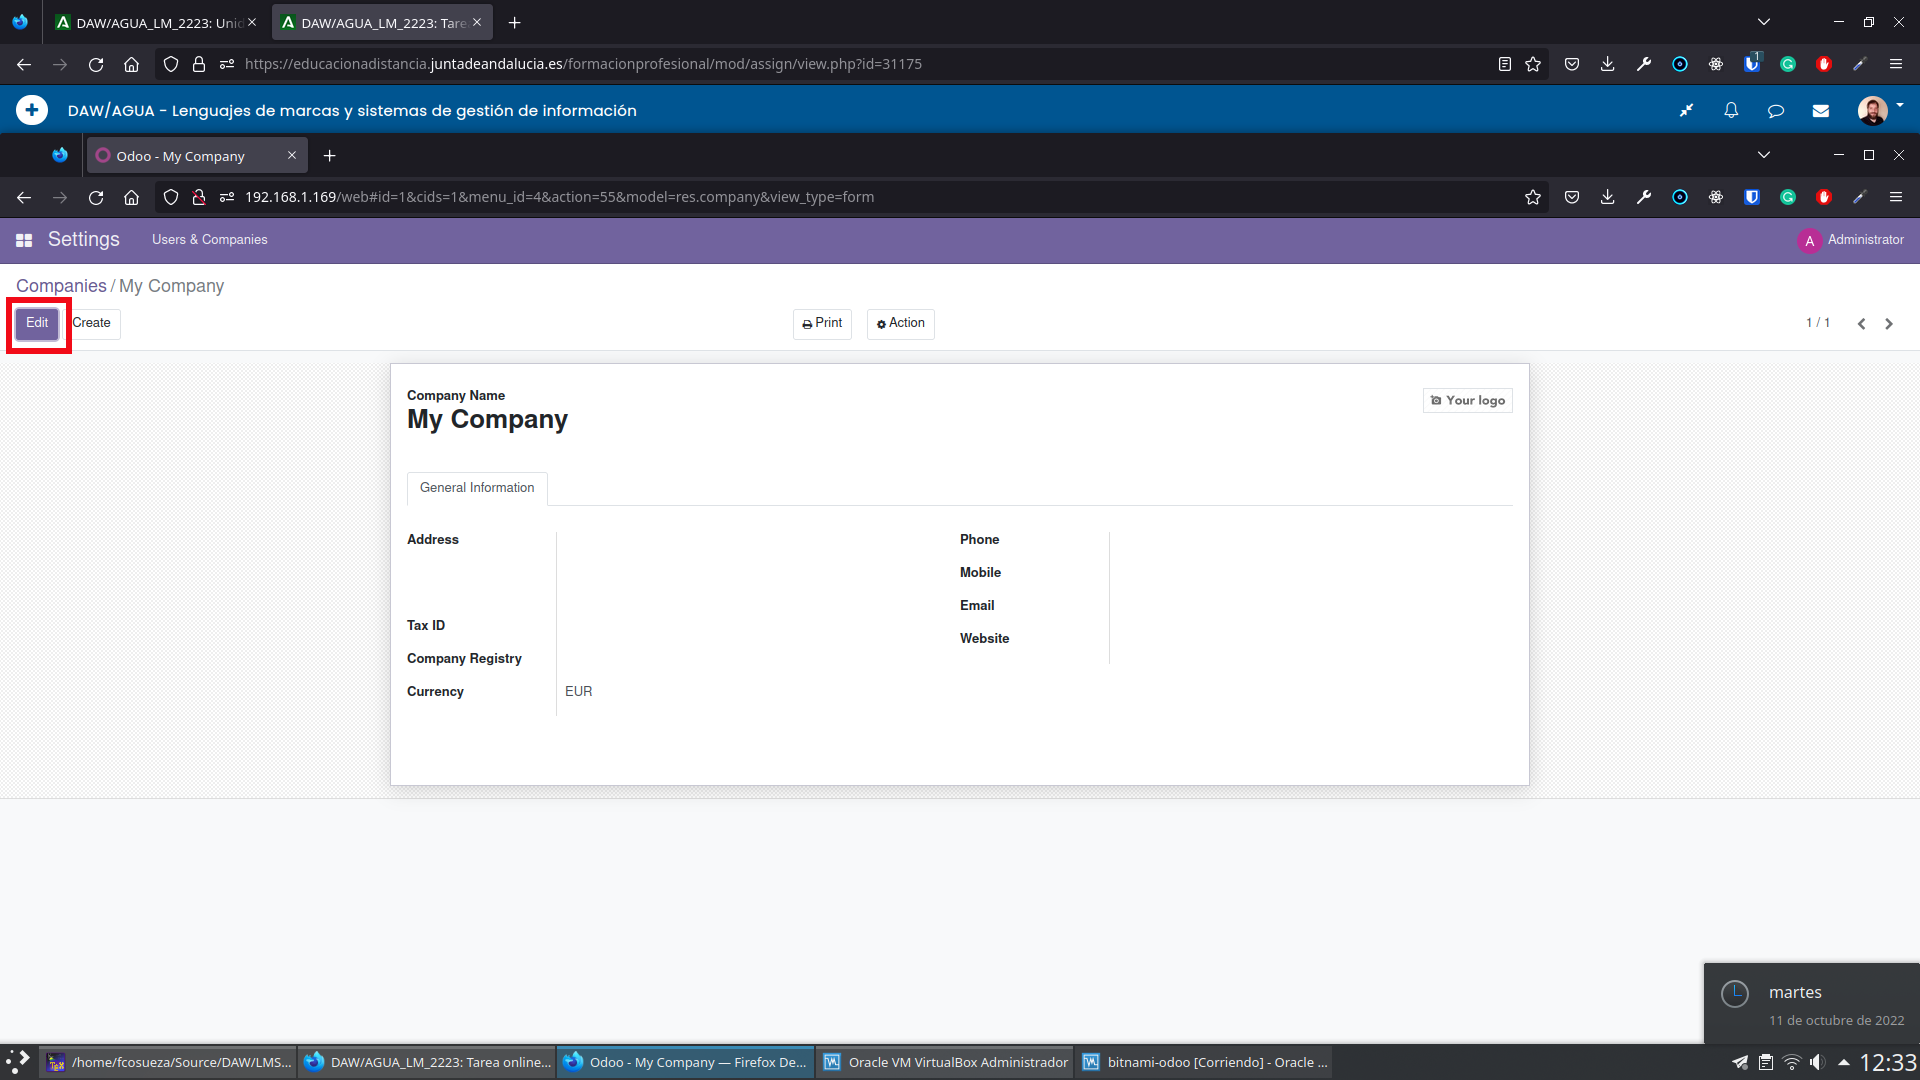
\includegraphics[scale=0.25]{odoo-comp-02.png}
        \caption{Ficha de compañía}
    \end{figure}

    \item Se nos mostrará una pantalla con donde podremos editar los diferentes datos de nuestra compañía. Una vez que hayamos completado el formulario, pulsamos el botón \textbf{Save} y los datos se habrán actualizado.

        \begin{figure}[h]
        \centering
        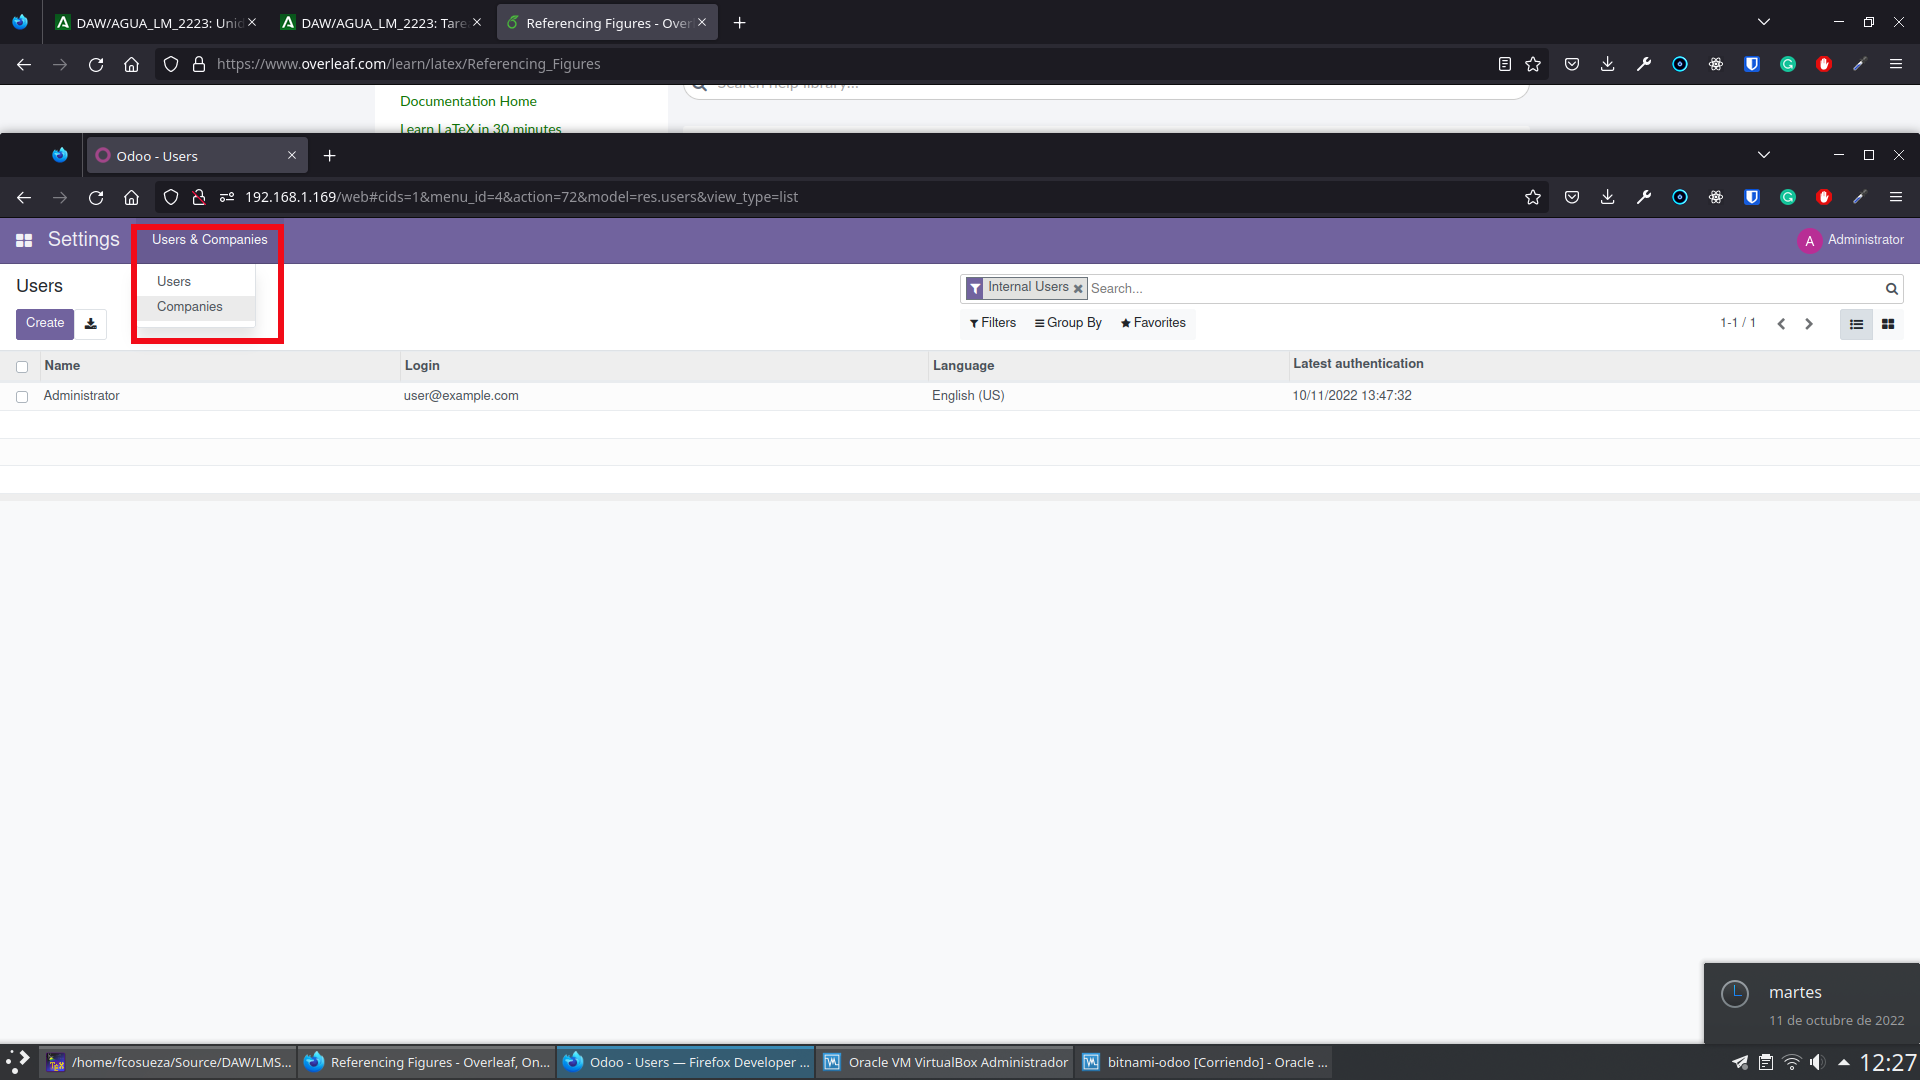
\includegraphics[scale=0.25]{odoo-comp-01.png}
        \caption{Formulario datos de la compañía}
    \end{figure}
\end{enumerate}

\section{Creación de Usuarios}






% Bibliography

\newpage
\bibliography{citas}
\bibliographystyle{unsrt}

\end{document}